\chapter{欧氏空间中的Plateau问题}
\newcommand{\FG}{{\mathcal{F}_\gamma}}
\newcommand{\FGG}{{\mathcal{F}_{\Gamma, g}}}
\newcommand{\fgg}{{\mathcal{F}_{\Gamma, g}}}
\newcommand{\AG}{{\mathbb{A}_\gamma}}
\renewcommand{\EG}{{\mathbb{E}_\gamma}}
\renewcommand{\E}{{E}}
\newcommand{\Polygon}{{\mathcal{P}}}
\renewcommand{\D}{{\mathbb{D}}}
\newcommand{\EE}{{\mathbb{E}}}
\renewcommand{\AA}{{\mathbb{A}}}
\renewcommand{\HH}{{\mathbb{H}^2}}
\newcommand{\HC}{{\overline{\mathbb{H}}^2}}
\newcommand{\PTT}[1]{{\partial_\theta #1}}
\newcommand{\RR}{{\overline{\mathbb{R}}}}
\newtheorem*{plateauproblem*}{Plateau问题}
\section{The Disk Case}
本章中, 我们回到最开始的问题:
\begin{plateauproblem*}
    给定简单闭曲线$\gamma \subset \R^3$, 是否存在以$\gamma$为边界的面积最小的曲面? 即, 寻找曲面$\Sigma, \partial \Sigma = \gamma$, 使得对于任意满足$\partial \Sigma' = \gamma$的曲面$\Sigma'$, 都有
    \begin{equation*}
        \Area(\Sigma) \le \Area(\Sigma')
    \end{equation*}
\end{plateauproblem*}
在本章, 按照Douglas和Rado的方法, 我们将给出Plateau问题的肯定的回答. 关于Douglas在Plateau问题上的工作的简介, 可以参考\cite{WorkofDouglas}.
\par 设$\gamma \subset \R^3$是简单闭曲线. 记
\begin{equation}
    \begin{split}
        \FG=\{
            u \mid  u\in C(\overline{\D})\cap W_{loc}^{1,2}(\D,\R^3),
            u\mid_{\P \D}: \P \D \to \gamma \text{是单调单射}.
        \}
    \end{split}
\end{equation}
\begin{remark}
    称$u\mid _{\P \D}$是单调映射, 是指我们将$\gamma$沿任意点剪断后看作实轴上的一段线段,  $u$是通常意义下的单调映射.  这里之所以没有要求$u$是同胚, 是因为同胚在求极限后(一致收敛拓扑)不会被保持,  而单调性总是会被保持的. 
\end{remark}
解决Plateau问题的第一选择是:取$u_k \in \FG$使得$\Area(u_k(\D)) \to \AG$, 并证明$\{u_k\}$存在收敛子列. 然而这种思路有两个问题需要解决:
\begin{enumerate}
    \item 我们可以改变$u_k$在任意点$p$附近的值, 得到$\tilde{u}_k$, 使得$\tilde{u}_k$与$\tilde{u}_k(\mathbb{D})$与 $u_k(\D)$相差"细长"的管状区域, 如图. 这样得到的$\tilde{u}_k$仍然是面积最小的列. 但是这样的列无法在通常的意义下收敛.  如图\eqref{figure_area_minimizing}所示.
    \begin{figure}[ht]
        \centering
        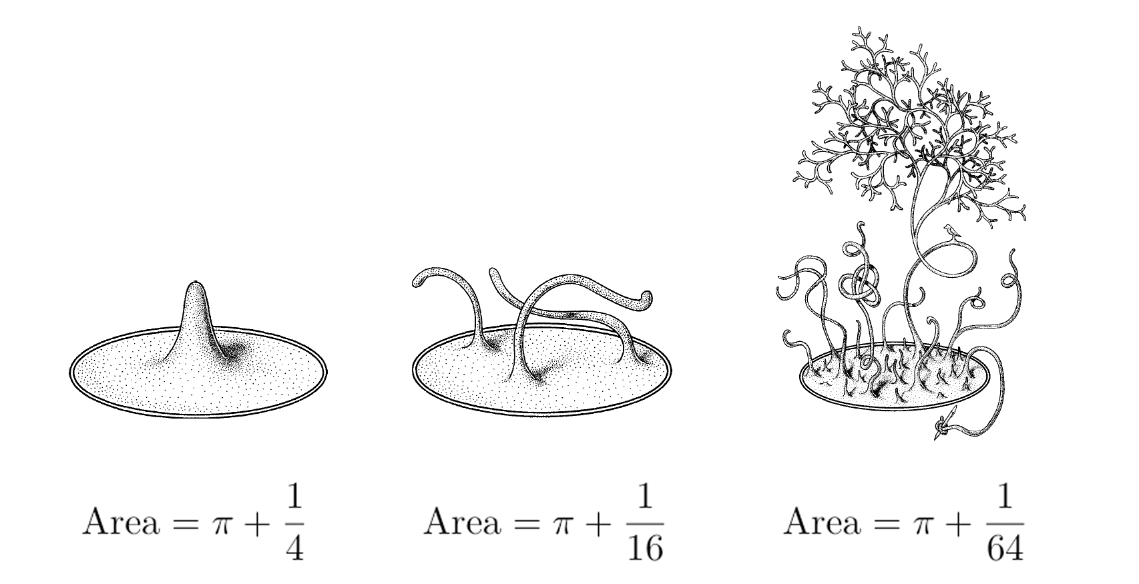
\includegraphics[scale=0.7]{images/area_minimizing.png}
        \caption{面积最小列, 但是没有收敛子列. 图片取自\cite{Morgan}}
        \label{figure_area_minimizing}
    \end{figure}
    \item 第二个问题是面积泛函是与参数选取无关的, 这意味着选取$\{u_k\}$后, 对于任意的微分同胚$\phi_k: \D \to \D$, $\Area(u_k\circ \phi_k(\D))= \Area(u_k(\D))$. 这种情况下, 我们也很难得到收敛子列.
\end{enumerate}
为了解决上面的问题, 我们将使用能量泛函而不是面积泛函. 当然, 首先我们需要说明的是, 对能量泛函求最小值和对面积泛函求最小值这两个问题是等价的(虽然对于能量泛函, 上述两个问题仍然存在, 但是我们较好的解决该问题的方法). 关于Plateau问题的解, 可以参考\cite{JostTwo}. 关于Plateau问题发展的历史, 可以参考\cite{FomenkoI}, \cite{FomenkoII}.
\begin{theorem}[Rado-Douglas] \label{rado_douglas}
    设$\gamma \subset \R^3$是可求长的Jordan曲线. 则存在映射$u \in \FG$使得 $\forall v \in \FG$, 
    \begin{equation}
        \Area(u(\D))\le \Area(v(\D)).
    \end{equation}
\end{theorem}
对于任意$u \in \FG$, 其面积与能量分别定义为
\begin{align}
    &\Area(u)=\int_\D\abs{u_x\wedge u_y} \\
    &\E(u)=\frac{1}{2}\int_\D\abs{u_x}^2+\abs{u_y}^2
\end{align}
简单计算可知
\begin{equation}\label{AleE}
    \Area(u)=\int_\D \sqrt{\abs{u_x}^2\abs{u_y}^2-\inner{u_x}{u_y}^2} \le \frac{1}{2}\int_\D \abs{u_x}^2+\abs{u_y}^2 \le\E(u).
\end{equation}
并且等号成立, 当且仅当$\abs{u_x}=\abs{u_y}, \inner{u_x}{u_y}=0$.
\par 记
\begin{align}
    &\AG=\inf\{\Area(v)\mid v \in \FG\}.\\
    &\EG=\inf \{\E(v)\mid v \in \FG\}.
\end{align}
\begin{definition}
    如果$u \in W^{1,2}(\mathbb{D},\R^3)$几乎处处满足$\inner{u_x}{u_y}=0$并且$\abs{u_x} = \abs{u_y}$, 则称$u$是几乎共形的.
\end{definition}
\begin{lemma}\label{ageg}
    $\AG=\EG$, 并且如果$u \in \FG$取到$\EG$, 则$u$是几乎共形的.
\end{lemma}
\begin{proof}
    由不等式\eqref{AleE}可知, $\AG \le \EG$.
    \par 对于反方向的, 设$u\in \FG$ 且$\Area(u) \le \AG + \epsilon$. 首先设$u$是浸入, 即$du$处处非退化. 设$(\D,g)$为$u$作用下的拉回度量, 即$g=du^*dx^2$, 由等温坐标的存在性可知, 存在光滑同胚$\phi: \D \to \D$使得$\phi$是$\mathbb{D} \to (\D,g)$ 之间的共形映射, 即$d\phi ^* g=\lambda^2dx^2$. 而$u\circ \phi$是共形浸入, 则有
    \begin{equation}
        \AG+\epsilon\ge \Area(u)=\Area(u\circ \phi)=\E(u\circ \phi) \ge \EG
    \end{equation}
    如果$du$有奇点, 那么我们定义$u^s: \D \to \R^5$, $u^s(x,y)=(u,sx,sy)\in \R^5$. 则$du^s$是非退化的. 像上面一样, 通过$u^s$拉回的度量为$du^*g_{\R^3}+s^2(dx^2+dy^2)$. 显然地, 
    \begin{equation}
        \Area(u^s)=\int_\D \det (du^*g_{\R^3}+s^2I)  \to \Area(u).
    \end{equation}
    \begin{equation}
        \E(u^s\circ\phi)=\int_\D \abs{(u^s\circ \phi)_x}^2+ \abs{(u^s\circ \phi)_y}^2 =\E(u\circ \phi)+s^2\E(\phi).
    \end{equation}
    因此, 当$s$足够小时, 我们有
    \begin{equation}
        \begin{split}
            \AG+2\epsilon \ge \Area(u)+\epsilon & \ge \Area(u^s\circ \phi)  \\
            &= \E(u^s\circ \phi)  \to \E(u\circ \phi) \\
            &\ge \EG.
        \end{split}
    \end{equation}
    若$E(u)=\EG$, 则$E(u)= \EG = \AG \le \Area(u)$, 则$E(u)=\Area(u)$. 由不等式\eqref{AleE}可知, $u$是几乎共形的.
\end{proof}
\begin{lemma}[Courant-Lebesgue引理] \label{courant_lebesgue}
    设$f \in W^{1,2}(\D,\R^3)$, $E(f) \le K$. 设$0 < \delta < 1$, $p \in \mathbb{D}$. 则存在$\rho \in (\delta, \sqrt{\delta})$ 使得$f\mid_{\P B(p,\rho) \cap \D}$是绝对连续的, 且$\forall z_1,z_2 \in \P B(p,\rho) \cap \D$, 成立 
    \begin{equation}
        \int_{\P B \cap \D} f_\theta^2 d\theta \le \frac{4K}{\log \rec{\delta}}
    \end{equation}
    以及
    \begin{equation}
        \abs{f(z_1)- f(z_2)} \le (8K\pi)^{\frac{1}{2}}(\log \frac{1}{\delta})^{-\frac{1}{2}}.
    \end{equation}
\end{lemma}
\begin{proof}
    在$p$点处引入极坐标$(r,\theta)$. 由于$f \in W^{1,2}$, 则几乎对于所有的$r$, $f$关于$\theta$是绝对连续的.  则Cauchy不等式, 
    \begin{equation}
        \begin{split}
            \abs{f(z_1)-f(z_2)} &\le \int_{\P B \cap \D} \abs{f_\theta(re^{i\theta})}d\theta \\
            & \le \sqrt{2\pi} (\int_{\P B\cap \D} f^2_\theta d\theta)^{\frac{1}{2}}.
        \end{split}
    \end{equation}
    而由于在极坐标下, $Df=f_r \P_r + \frac{1}{r^2}f_\theta \P_\theta$, 则
    \begin{equation}
        \int_{B \cap \D} (f_r^2 + \frac{1}{r^2}f_\theta^2)r drd\theta \le 2K.
    \end{equation}
    取$\rho$使得$\int_{\P B \cap \D} f^2_\theta(\rho e^{i\theta})$取到(几乎)最小, 则有
    \begin{equation}
        \int^{\sqrt{\delta}}_\delta \int_{\P B \cap \D}\frac{1}{r^2}f^2_\theta(\rho e^{i\theta}) rd\theta dr \le 2K.
    \end{equation}
    因此, 
    \begin{equation}
        \abs{f(z_1)-f(z_2)} \le \sqrt{2\pi} \frac{2K}{ \int^{\sqrt{\delta}}_\delta \frac{1}{r}} = \sqrt{8K\pi}(\log \frac{1}{\delta})^{-\frac{1}{2}}.
    \end{equation}
\end{proof}
\begin{remark}
    Courant-Lebesgue引理在实际应用中, 我们只会在靠近边界的地方应用该引理. 将单位圆盘换成任意有限拓扑型的黎曼面$\Sigma$, 结论都是成立的(只需要取$\delta \le C=C(\Sigma)$). 后面在解决一般拓扑型的Plateau问题时, 我们还会多次用到Courant-Lebesgue引理.
\end{remark}
\begin{lemma}\label{three_point}
    设$p_1,p_2,p_3  \in \partial \D$是三个不同的点. 则对于任意三个点$\forall p'_1, p'_2, p'_3$, 存在唯一的共形同胚$\alpha: \D \to \D$使得$\alpha(p_i)=p'_i$. (假设$p_i, p'_i$在$\P \D$上都按逆时针排列)
\end{lemma}
\begin{proof}
    见任意复分析教材.
\end{proof}
\begin{lemma}\label{cut_curves}
    设$\gamma \subset \R^3$是长度有限的Jordan曲线, 则$\forall \epsilon > 0$, 存在$\lambda>0$使得$\forall p,q \in \gamma$, 如果$d(p,q)< \lambda$, 那么$\gamma-\{p,q\}$的两条曲线中, 只有一条的
    %直径(作为集合的直径)可以大于$\epsilon$. 
    长度可以大于$\epsilon$. 
\end{lemma}
\begin{proof}
    略.
\end{proof}
现在, 固定三个点$p_i \in \P D$, $q_i \in \gamma$. 设$K > 0$, 记
\begin{equation}
    \FG^K=\{u \in \FG\mid E(u) \le K, u(p_i)=q_i\}.
\end{equation}
\begin{lemma} \label{boundary_equicontinuous}
    $\FG^K\mid_{\P D}$是等度连续的.
\end{lemma}
\begin{figure}[ht]
    \centering
    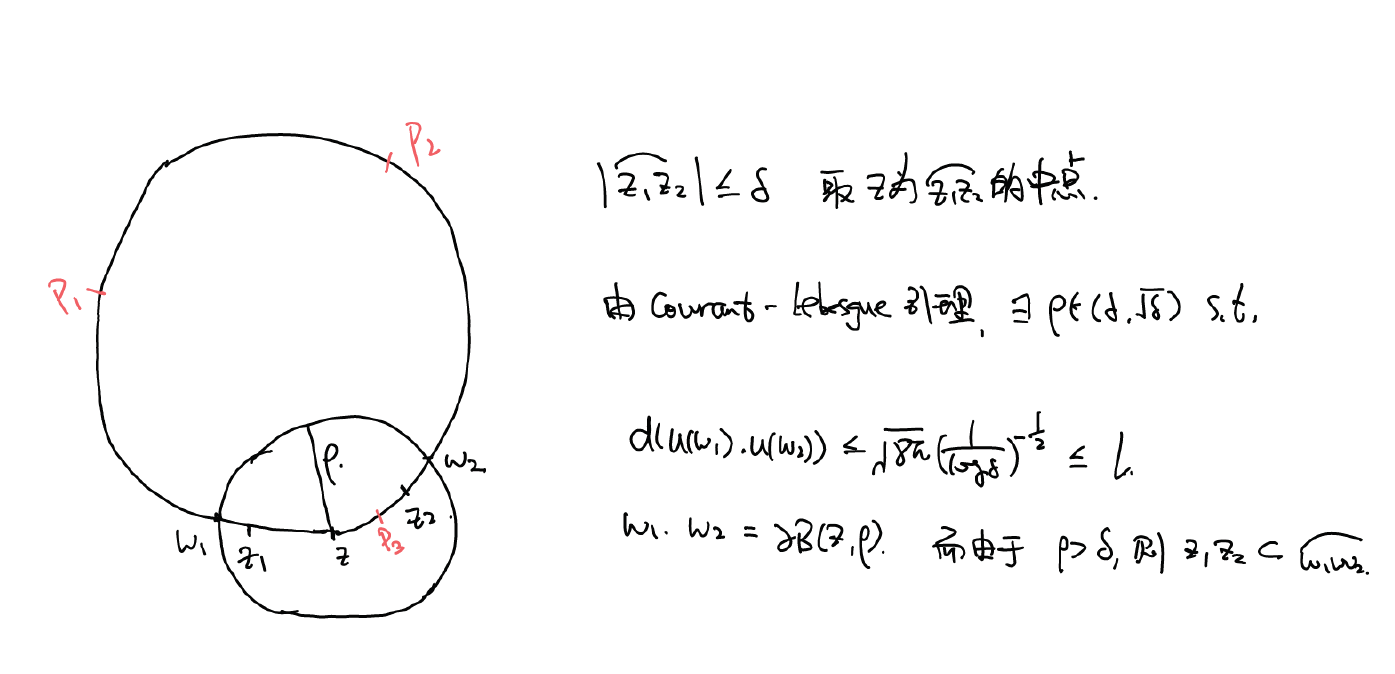
\includegraphics[scale=0.6]{images/courant_lebesgue.png}
    \caption{边界等度连续性}
    \label{equi_continuous}
\end{figure}
\begin{proof}
    我们选取$\epsilon$非常小, 使得$\gamma$中任意长度为$\epsilon$的曲线段都至多包含$\{q_i\}$中的一个点. 现在, 我们证明存在$\delta>0$, 使得如果$z_1,z_2 \in \P \D, \abs{z_1-z_2} \le \delta$, 则$\forall u \in \FG^K$, $\abs{u(z_1)-u(z_2)} \le \epsilon$.  
    \par 取$\delta$使得$(8K\pi)^{\rec{2}}(\log \rec{\delta})^{-\rec{2}} \le \lambda$, $\lambda$由引理\eqref{cut_curves}得到.  设$z_1,z_2 \in \P \D$.  设$\abs{z_1-z_2} \le \rec{\pi} \delta$, 用$\widehat{z_1z_2}$表示$\P \D - \{z_1,z_2\}$中较短的弧, 显然地, $\abs{\widehat{z_1z_2}} \le \delta$. 只要取$\delta$足够小, 就可以假设$\widehat{z_1z_2}$至多包含$\{p_i\}$中的一个点. 设$z$是弧$\widehat{z_1z_2}$的中点. 由引理\eqref{courant_lebesgue}, 存在$\rho \in (\delta, \sqrt{\delta})$使得$\forall u \in \FG^K$, 
    \begin{equation}
        d(u(w_1),u(w_2)) \le (8K\pi)^{\rec{2}}(\log \rec{\delta})^{-\rec{2}} \le \lambda.
    \end{equation}
    记$\{w_1,w_2\} = \P B(z,\rho) \cap \P \D$, 那么$u(w_1), u(w_2)$将$\gamma$分成两段, 其中较短的一段至多包含$\{q_i\}$中的一个点. 那么, 这一段的原像必定是$\widehat{w_1w_2}$.  而由于$\rho > \delta$, 则$z_1,z_2 \in \widehat{w_1w_2}$. 则$d(u(z_1),u(z_2)) \le \epsilon$.
\end{proof}
\begin{proof}[定理\eqref{rado_douglas}的证明]
    取$u_k \in \FG$ 且$E(u_k) \to \EG$. 由引理\eqref{three_point}, 存在$\phi_k$使得$u_k\circ \phi_k \in \FG^K$. 仍将$u_k\circ \phi_k$记为$u_k$.  用与$u_k$具有相同边界的调和函数替换$u_k$, 仍然记为$u_k$, 由于调和函数是能量最小的, 我们仍然有$E(u_k) \to \EG$.  由于$u_k$是调和的, 则
    \begin{equation}
        \max_{\D}\abs{u_k - u_l} = \max_{\P \D} \abs{u_k-u_l}.
    \end{equation}
    而根据引理\eqref{boundary_equicontinuous}, $u_k\mid_{\P \D}$ 包含一致收敛子列, 则$u_k$包含一致收敛子列. 设$u_k \to u$.  再选取$u_k$的子列, 使得$u_k \overset{\text{弱}W^{1,2}}{\longrightarrow} u$且$u_k \overset{L^2}{\longrightarrow} u$. 则由能量的下半连续性, 
    \begin{equation}
        E(u) \le \liminf E(u_k) \to \EG.
    \end{equation}
    最后, 由引理\eqref{ageg}, $\Area(u)=E(u)=\AG$.
\end{proof}
\ifcomment
    \begin{remark}
        如果没有三点正规化的话, 不影响等度连续性, 但是得到的极限可能是常值函数.
    \end{remark}
\fi
\section{The Annulus Case}
现在, 我们考虑复杂一点的情况. 设$\Gamma=\gamma_1 \cup \gamma_2$是两条简单闭曲线的并. 是否存在以$\Gamma$为边界的极小曲面?  
\par 与圆盘的情况不同的是,  并不总是能找到以$\Gamma$为边界的极小曲面.  这里我们给出一个反例.  设$\Sigma$为Catenoid, 即$\Sigma=\{\cosh^2 z = x^2+y^2\}$.  设$\Sigma_a= a\Sigma$.  那么, 当$a \to +\infty$时,  $\Sigma_a \to \emptyset$.  $a\to 0$时, $\Sigma_a \to 2\{z=0, x^2+y^2\ne 0\}$.  简单计算易知,  存在锥体$C_\lambda=\{x^2+y^2< \lambda^2z^2\}$使得$C_\lambda\cap \Sigma=\emptyset$.  而由于$C_\lambda$在相似变换下是不变的, 则$\forall \Sigma_a \cap C_\lambda = \emptyset$.  分别记$C^+_\lambda=C_\lambda \cap \{z>0\}$, $C^-_\lambda=C_\lambda \cap \{z<0\}$. 
\begin{figure}[ht]
    \centering
    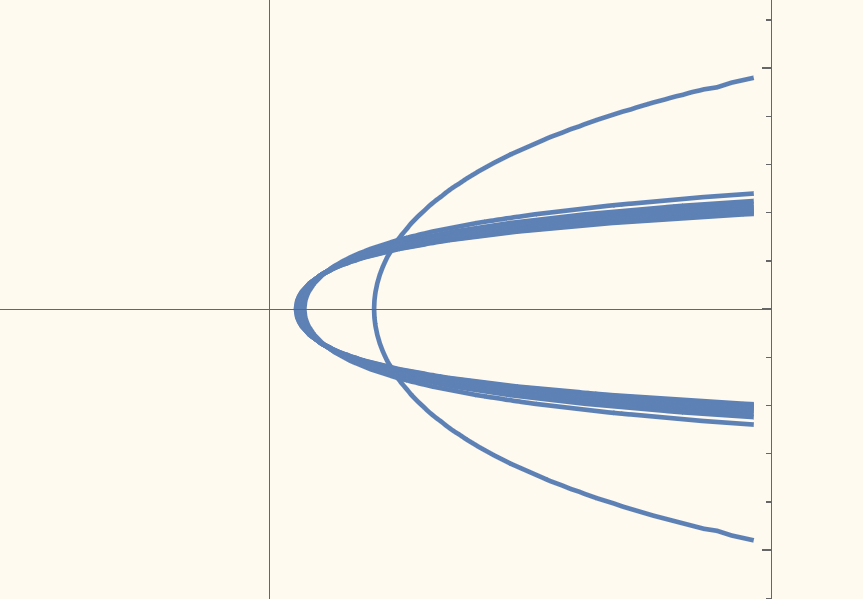
\includegraphics[scale=0.4]{images/sequence_of_catenoid.png}
    \caption{$\Sigma_a$与$C_\lambda$没有交集.}
    \label{label}
\end{figure}
%\lstinputlisting[language=Mathematica]{mathematica/sequence_of_catenoid.m}
\begin{definition}
    设$\Sigma$是二维流形. 称$\Sigma$是双连通的, 如果$\Sigma$同胚于$\{1< \abs{z}< 2\}$.  双连通曲面有时我们也会称为annulus型曲面.
\end{definition}
\begin{proposition}
    设$\Gamma=\gamma_1 \cup \gamma_2$, $\gamma_1 \subset C^+_\lambda, \gamma_2 \subset C^-_\lambda$. 则不存在以$\Gamma$为边界的双连通极小曲面.
\end{proposition}
\begin{proof}
    设这样的极小曲面存在, 记为$M$.  显然地, $a \to 0$时,  $\Sigma_a \cap M \ne \emptyset$.  $a \to \infty$时, $\Sigma_a \cap M = \emptyset$. 那么存在$a$使得$\Sigma_a$恰好与$M$相切且位于$M$的同一侧, 这将与最大值原理矛盾.
\end{proof}

在此, 我们指出, 在解决给定拓扑型的Plateau问题时, 我们所会碰到的核心困难在于拓扑型的退化. 如图\eqref{figure_annulus_minimizing}我们要寻找由两个圆盘围出的同胚于环面的极小曲面(图一图二均为两个环面, 且面积变小. 图三为两个圆盘). 当我们取面积递减的曲面序列的时候, 虽然所取的每一个曲面都同胚于环面, 但是最终得到的极限却是两个圆盘. 这种现象便是拓扑型的退化.即, 取极限后无法保证得到的曲面的拓扑是我们想要的.
\begin{figure}[ht]
    \centering
    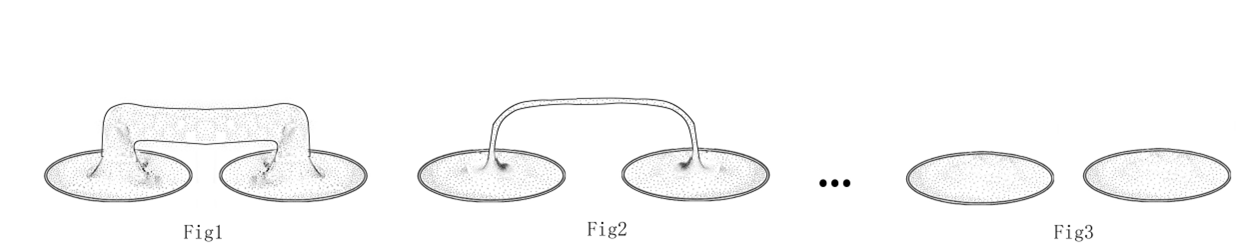
\includegraphics[scale=0.8]{images/annulus_minimizing.png}
    \caption{拓扑型的退化}
    \label{figure_annulus_minimizing}
\end{figure}

\par 解决annulus型的Plateau问题, 与disk型的另一个区别在于, 在选取参数域的时候, 由于所有的单连通区域(除了$\mathbb{C}$及$\S^2$)都是共形等价的, 我们可以假设参数域就是单位圆盘$\D$. 然而在双连通的情况, 由定理\eqref{uniformization_annulus}, 双连通域之间并不一定共形等价, 这样我们在选取参数域的时候就多了一个参数(区域的共形模, 参考定义\eqref{conformal_modulus}).  
\begin{remark}
    $B_{1,e^s}=\{1<\abs{z}< e^s\}$与$\S^1\times (0, s)\subset \R^3$是共形等价的,  我们将选取$\S^1\times (0,s)$形的区域作为参数域.
\end{remark}
下面介绍的两个引理\eqref{boundary_energy}, \eqref{fill_hole}起到的都是``补洞''的作用.
\begin{lemma} \label{boundary_energy}
    设$\phi: \S^1 \to \R$是绝对连续的,  设$u\in C(\D)$是调和函数并且$u\mid_{\P \D}=\phi$. 则
    \begin{equation}
        \int_{\D} \abs{\nabla u}^2dxdy \le \int_{\S^1} \abs{\phi_\theta}^2d\theta.
    \end{equation}
\end{lemma}
\begin{proof}
    设$(r,\theta)$是极坐标. 设$c_n=\rec{2\pi}\int_{\S^1} \phi(\theta)e^{-i n \theta}d\theta$. 则$u, u_r$具有展开式
    \begin{align}
        &u(r,\theta)=\sum_{-\infty}^{+\infty}c_n r^{\abs{n}}e^{in\theta}, \label{fourier_u} \\
        &u_r(r,\theta)=\sum_{-\infty}^{+\infty}c_n\abs{n} r^{\abs{n}-1}e^{in\theta}. \label{fourier_ur}
    \end{align}
    由于$u$是实函数, 由$c_n=\bar{c}_{-n}$. 由散度定理, 并将\eqref{fourier_u},\eqref{fourier_ur}代入计算可知
    \begin{equation}
        \begin{split}
            \int_{{\abs{z}\le r}}\abs{\nabla u}^2dxdy & =\int_{\{\abs{z}=r\}}uu_rd\theta\\
            &=2\pi \sum_{-\infty}^{+\infty}\abs{n}r^{2n}\abs{c_n}^2.
        \end{split}
    \end{equation}
    另外, 由于$L^2$函数的傅立叶级数$L^2$收敛, 则有
    \begin{equation}
        \int_{\S^1} \abs{u_\theta}^2 = 2\pi\sum_{-\infty}^{+\infty} \abs{n}^2\abs{c_n}^2.
    \end{equation}
    令$r \to 1$即可.
\end{proof}
\begin{lemma} \label{fill_hole}
    设 $\delta <1$. 定义
    \begin{equation}
        \eta_\delta(r)=\left\{
            \begin{aligned}
                &1 \s r \ge \sqrt{\delta}, \\
                &1+\frac{\log \sqrt{\delta}- \log r}{ \log \sqrt{\delta}} \s \delta \le r \le \sqrt{\delta}\\
                &0 \s r \le \delta
            \end{aligned}
            \right.
    \end{equation}
    设$u \in W^{1,2}(\Sigma) \cap C(\Sigma)$. 定义
    \begin{equation}
        u_\delta(z)=\left\{
            \begin{aligned}
                & u(z) \s \abs{u(z)-p} \ge \sqrt{\delta} \\
                & p+ \eta_\delta(\abs{u(z)-p})(u(z)-p)
            \end{aligned}
        \right.
    \end{equation}
    则当$\delta \to $时, $E(u_\delta) \to E(u)$.
\end{lemma}
\begin{figure}[h]
    \centering
    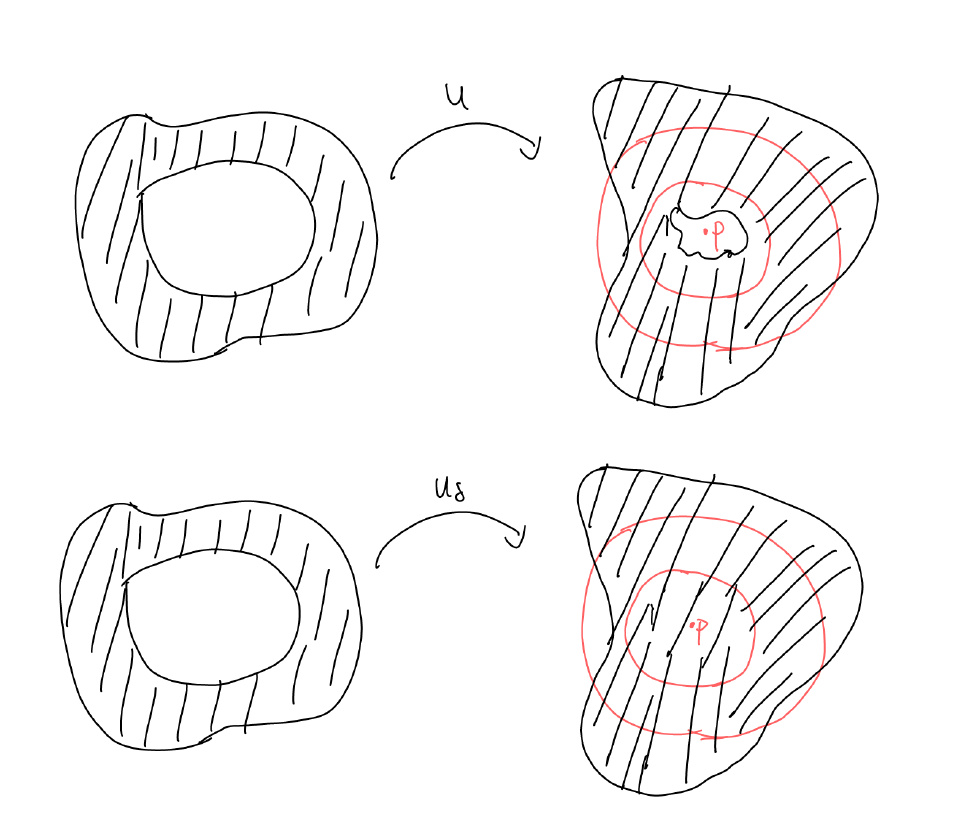
\includegraphics[scale=0.5]{images/contraction.png}
    \caption{$u_\delta$填补了$u$的像中的``空洞"}
    \label{aaaanonlabel}
\end{figure}

\begin{proof}
    设$\Omega_\delta=\{\abs{u(z)-p} < \sqrt{\delta}\}$. 则 $E(u_\delta)=E(u,\Sigma-\Omega_\delta)+E(u_\delta, \Omega_\delta)$. 我们计算第二项.
    \begin{equation}
        \begin{split}
            E(u_\delta, \Omega_\delta) & =\rec{2}\int_{\Omega_\delta} {\eta'}^2(\abs{u(z)-p})\abs{Du}^2+\eta^2(\abs{u(z)-p}) \abs{Du}^2 dv_g\\
            &\le \rec{2}\int_{\Omega_\delta} \frac{\abs{Du}^2}{(\log\sqrt{\delta}\delta)^2} +\abs{Du}^2dv_g
        \end{split}
    \end{equation}
    因此, 
    \begin{equation}
        \abs{E(u)-E(u_\delta)} \le \frac{1}{\delta\log\sqrt{\delta}}\int_{\Omega_\delta} \abs{Du}^2dv_g \to 0.
    \end{equation}
\end{proof}
对于annulus型的Plateau问题, Douglas的结果可以陈述为:
\begin{theorem}\label{theorem_douglas_annulus}
    设$\Gamma= \gamma_1 \cup \gamma_2 \subset \R^3$是两条不相交的简单闭曲线的并. 设存在以$\Gamma$为边界的双连通曲面$M$使得
    \begin{equation} \label{douglas_condition_annulus}
        \Area(M) < \AA_{\gamma_1}+\AA_{\gamma_2}.
    \end{equation}
    则存在以$\Gamma$为边界的双连通的极小曲面.
\end{theorem}
\begin{proof}
    设$u_k: \Sigma \to \R^3$, $E(u_k) \to \EE_{\Gamma}$.  记$K=\EE_{\Gamma}+1 < +\infty$. 这里, $\Sigma_k = \S\times (0,s_k)$. 不失一般性, 可设$E(u_k) \le K$. 现在,我们证明: 存在子列使得 $s_k \to s >0$.  $\Sigma_k$上的参数记为$(\theta,r)$. $\theta \in \S^1, r \in (0,s_k)$.
    \begin{claim}
        $\{s_k\}$有严格正的下界.
        \begin{subproof}
            记$d=d(\gamma_1,\gamma_2)>0$. $\forall \theta \in \S^1$, 设$\alpha$ 为直线$\theta \times (0, s_k)$. 则$u\circ\alpha$是连接$\gamma_1,\gamma_2$的一条曲线. 显然地, $l_{u_k(\alpha)} \ge d$. 则由Cauchy不等式
            \begin{equation}
                d^2 \le (\int^{s_k}_0 \abs{du_k \alpha'} ds)^2 \le s_k \int^{s_k}_0 (\PTT{u_k})^2dr.
            \end{equation}
            于是, 有
            \begin{equation}\label{annulus_small_energy}
                \frac{2\pi d^2}{s_k} \le \int_{\S^1}\int^{s_k}_0 (\PTT{u_k})^2 drd\theta \le E(h) \le K.
            \end{equation}
            则$s_k \ge \frac{2\pi d^2}{K}$.
        \end{subproof}
    \end{claim}
    \begin{claim}
        $\{s_k\}$有上界(不等于$+\infty$).
        \begin{subproof}
            反证法.  设$s_k \to +\infty$. 由于$\E(u_k) \le K$,  则存在$\rho_k \in (0, s_k)$使得
            \begin{equation}
                s_k\int_{\S^1 \times \{\rho_k\}} (\PTT{u_k})^2(\theta,\rho_k) d\theta \le K.
            \end{equation}
            \begin{figure}[!h]
                \centering
                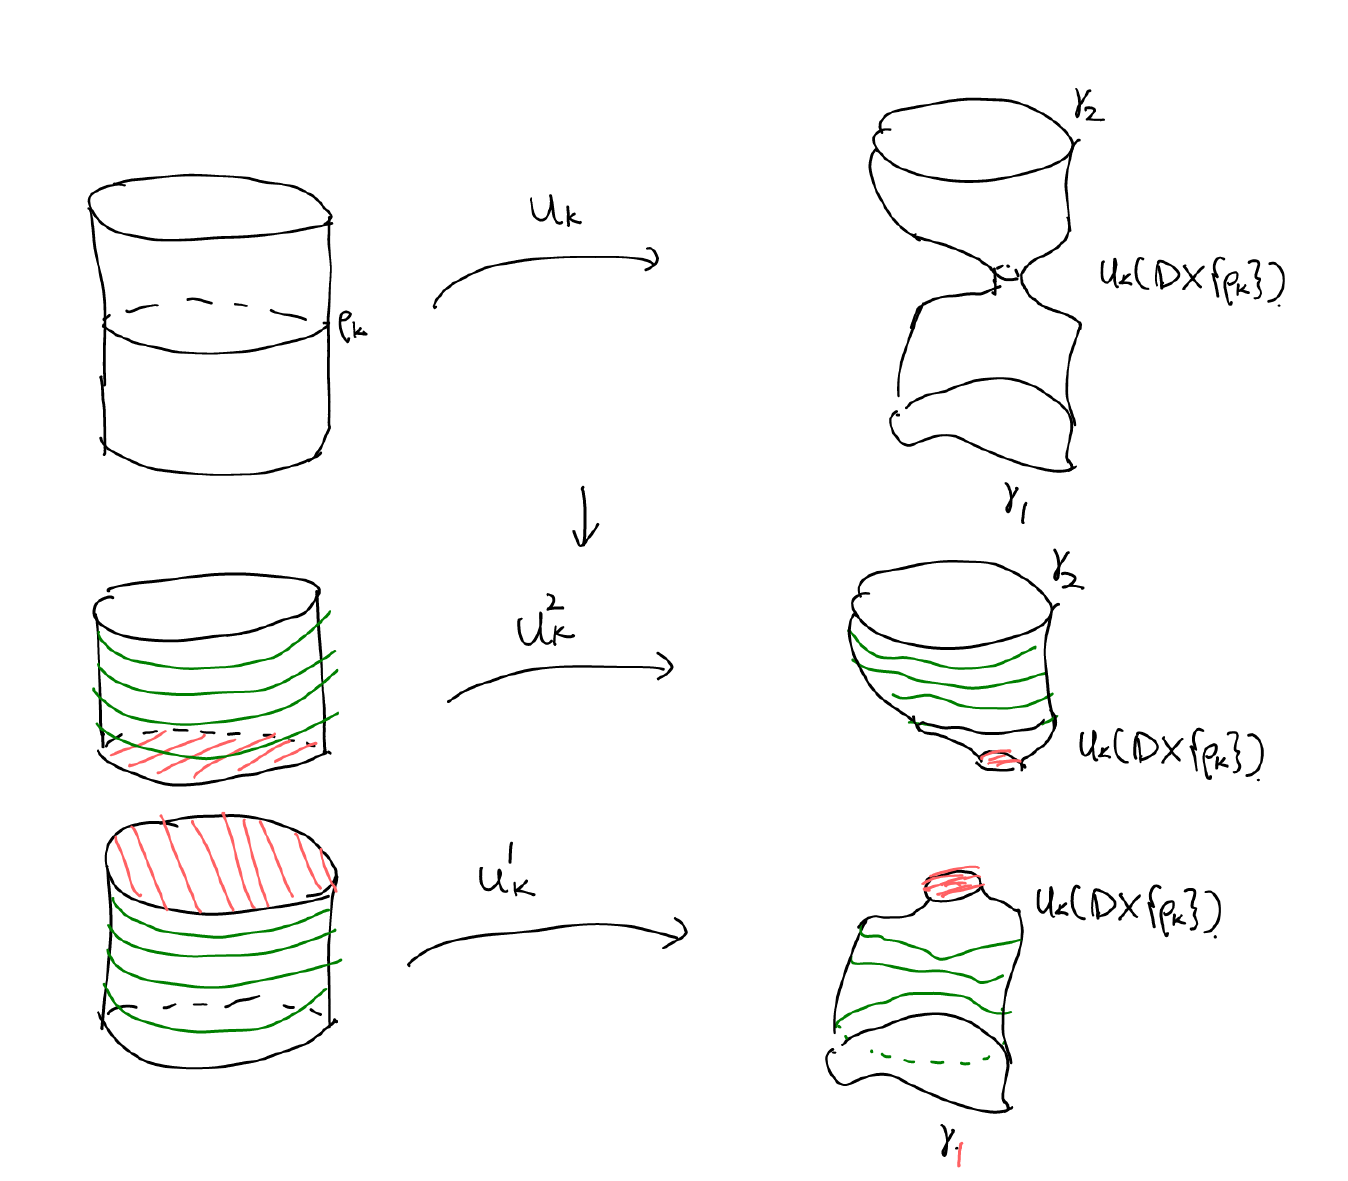
\includegraphics[scale=0.6]{images/closed_degenerate.png}
                \caption{曲线的退化}
                \label{closed_degenerate}
            \end{figure}
            则有$\int_{\S^1\times \{\rho_k\}} (\PTT{u_k})^2(\theta,\rho_k) d\theta  \to 0$. 实际上这意味着拓扑型的退化. 设$\gamma$为曲线$\S^1 \times \{\rho_k\}$并取其弧长参数, 则由Cauchy不等式,
            \begin{equation}
                l_\gamma = \int_\gamma\abs{\gamma'}ds \le (2\pi\int_\gamma \abs{\gamma'}^2ds^2)^\rec{2} \to 0.
            \end{equation}
            这意味着出现了图\eqref{figure_annulus_minimizing}中的情况.  现在我们利用Douglas条件\eqref{douglas_condition_annulus}来说明这是不可能发生的.
            记$\D_{\rho_k}=\D \times \{\rho_k\}$. 现在以$u_k(\rho_k,\theta)$为边界值, 由引理\eqref{boundary_energy}可知, 存在函数$f_k: \D_{\rho_k} \to \R^3$使得$E(f_k) \to 0$.  定义
            \begin{equation}
                \Sigma^1_k= \S^1 \times (0,\rho_k) \cup \D_{\rho_k},\s \Sigma^2_k=\S^1\times (\rho_k,s_k) \cup \D_{\rho_k}.
            \end{equation}
            显然地, $\Sigma^1_k, \Sigma^2_k$都是单连通的. 现在我们定义两个新的映射:
            \begin{equation}
                {u}_k^1: \Sigma^1_k \to \R^3.  \s  {u}_k^1=\left\{
                    \begin{aligned}
                        &u_k\s x \in \S^1 \times (0,\rho_k),\\
                        &f_k\s x \in \D_{\rho_k}.
                    \end{aligned}
                \right.
            \end{equation}
            \begin{equation}
                {u}_k^2: \Sigma^2_k \to \R^3.  \s  {u}_k^2=\left\{
                    \begin{aligned}
                        &u_k\s x \in \S^1 \times (\rho_k, s_k),\\
                        &f_k\s x \in \D_{\rho_k}.
                    \end{aligned}
                \right.
            \end{equation}
            则$E({u}_k^1)+E({u}_k^2) \le E(u_k)+2E(f_k)$. 而显然地, ${u}_k^1(\P \Sigma^1_k) = \gamma_1$,${{u}}_k^2(\P \Sigma^2_k)= \gamma_2$. 则
            \begin{equation}
                \begin{split}
                    \AA_{\gamma_1}+\AA_{\gamma_2} = \EE_{\gamma_1}+\EE_{\gamma_2} & \le  \lim E({u}_k^1)+E({u}_k^2)  \\
                    &\le \lim E(u_k) + 2E(f_k) \to \EE_\Gamma=\AA_\Gamma.
                \end{split}
            \end{equation}
            这与条件\eqref{douglas_condition_annulus}矛盾.
        \end{subproof}
    \end{claim}
    设$\Sigma_k \to \Sigma = \S^1 \times (0,s)$. 同时, 通过变换$(x,r) \to (x,\frac{s_k}{s}r)$, 我们可以假设$u_k$定义在$\Sigma$上.
    \begin{claim}
        $u_k\mid_{\P \Sigma}$是等度连续的.
        \begin{subproof}
            我们只考虑$u_k\mid_{\S^1 \times \{0\}}$的等度连续性即可.  设$\epsilon_k \to 0$,  $\forall p \in \S^1 \times \{0\}$, 取$\delta_k>0$使得, 
            \begin{equation}
                \sqrt{8K\pi}(\log(\rec{\delta_k}))^{-\rec{2}} \le \epsilon_k.
            \end{equation}
            由Courant-Lebesgue引理\eqref{courant_lebesgue}, 存在$\rho_k \in (\delta_k,\sqrt{\delta_k})$使得
            \begin{equation} \label{betak_to_0}
                l_{u_k(\P B(p,\rho_k) \cap \Sigma)} \le \sqrt{8K\pi}(\log(\rec{\delta_k}))^{-\rec{2}} \le \epsilon_k.
            \end{equation}
            记$\beta_k=\P B(p,\rho_k) \cap \Sigma$. $\beta_k$的端点将$\S^1 \times \{0\}$分成两部分, 其中短的一部分记为$C_k'$, 长的部分记为$C_k''$. $u_k(\beta_k)$的两个端点将$\gamma_1$分成两部分, 其中短的记为$\gamma_{1k}'$, 长的记为$\gamma_{1k}''$(``长'', ``短''是在引理\eqref{cut_curves}意义下的). 如同引理\eqref{boundary_equicontinuous}的证明中一样, 由Courant-Lebesgue引理,  如果能说明$\forall k$, $u_k(C_k')=\gamma_{1k}'$, 那么$u_k$是等度连续的.  反证法. 设$u_k(C_k')=\gamma_{1k}'', u_k(C_k'')=\gamma_{1k}'$. 由引理\eqref{cut_curves}及不等式\eqref{betak_to_0}, $l_{u(\beta_k)\cup \gamma_{1k}'} \to 0$.  注意到, $u_k(\beta_k) \cup \gamma_{1k}'$实际上是$u_k(\Sigma)$的core curve(也就是$u_k(\Sigma)$基本群的生成元), 这意味着出现了图\eqref{figure_annulus_minimizing}中的情况. 现在我们将构造两个映射$u_{1k}, u_{2k}$, 这两个映射都定义在单连通区域上, 且分别将两个单连通区域的边界映为$\gamma_1, \gamma_2$. 
            \begin{figure}[ht]
                \centering
                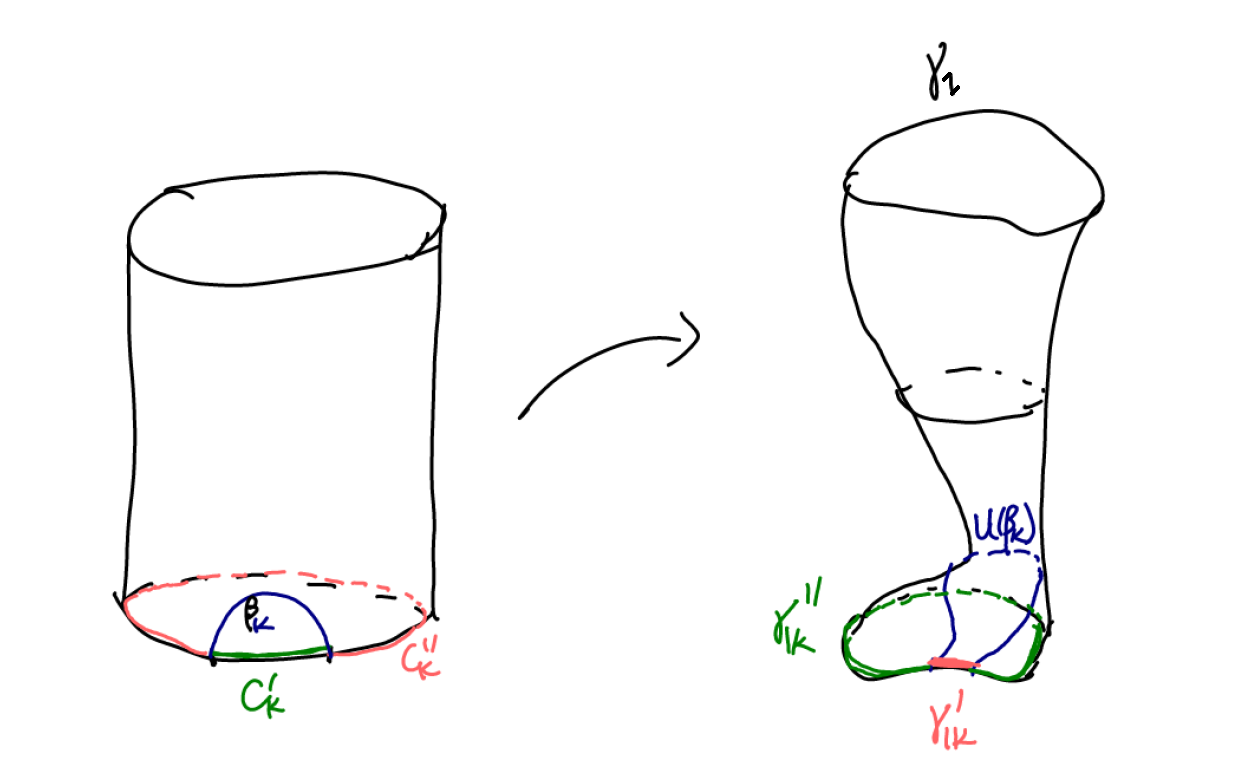
\includegraphics[scale=0.4]{images/pinch.png}
                \caption{设在$u_k$映射下, ``短''的弧被映射为``长''的弧}
                \label{pinch}
            \end{figure}
            \par 首先, 我们将曲面$\Sigma$沿着$\beta_k$剪开, 其中包含边界$\S^1\times \{s\}$的部分记为$\Sigma_k''$, 由$\beta_k$及$C_k'$围出的区域记为$\Sigma_k'$. 在$\Sigma_k''$的边界$C_k''\cup \beta$上, 粘贴上一个圆盘, 这样就得到了一个单连通区域, 记为$\tilde{\Sigma}_k''$.  %现在我们分别在$\Sigma_k'$及$\tilde{\Sigma}_k''$上定义两个映射.
            \par 取$q \in \R^3$使得$d(q, u_k(\beta_k) \cup \gamma_{1k}') < 2\epsilon_k$.  将引理\eqref{fill_hole}应用到$u_k, 2\epsilon_k, q$上(取$u=u_k, p=q, \delta=\epsilon_k$), 得到新的映射记为$u_{2k}$. 注意到$u_{2k}$将$\beta_k \cup C_k''$的邻域映射到点$q$. 在$\tilde{\Sigma}''_k-\Sigma''_k$上将$u_{2k}$定义常值$q$, 那么就得到了$u_{2k}: \tilde{\Sigma}_k'' \to \R^3, u_{2k}({\P \tilde{\Sigma}_k''})=\gamma_2$.
            \begin{figure}[ht]
                \centering
                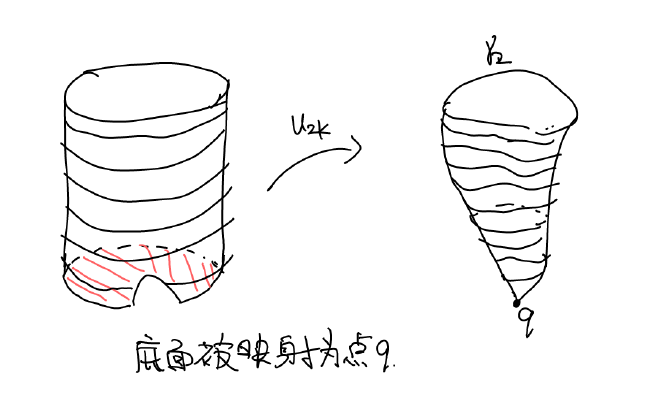
\includegraphics[scale=0.7]{images/u2k.png}
                \caption{$u_{2k}$}
                \label{u2k}
            \end{figure}
            \par  现在我们定义$u_{1k}$. 由于$\Sigma_k'$是单连通的, 我们将$\Sigma_k'$共形映射为下半单位圆盘, 并将$\beta_k$映射为$\{\abs{z}=1\} \cap \D$.  设$\gamma_{1k}'$的长度为$l_k$, 取$\gamma_{1k}'$的弧长参数化, 现在我们定义$\phi_k: \P \D \cap \{\Im(z)>0\} \to \R^3$, 对于$z \in \S^1 \cap \{\Im(z) >0\}$, 记$\theta(z)=\text{Arg}(z)$.
            \begin{equation}
                \phi_k=\left\{
                    \begin{aligned}
                        & u_k(z) \s z \in \{\Im(z)=0\}, \\
                        & \gamma_{1k}'(\frac{l_k}{\pi}\theta(z)) \s z \in \S^1 \cap \{\Im(z)>0\}.
                    \end{aligned}
                \right.
            \end{equation}
            \begin{figure}[!h]
                \centering
                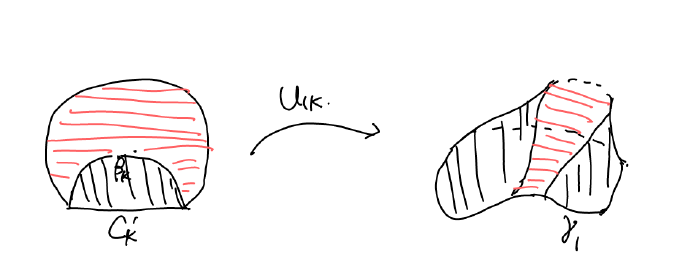
\includegraphics[scale=0.8]{images/u1k.png}
                \caption{$u_{1k}$}
                \label{u1k}
            \end{figure}
            由Courant-Lebesgue引理及$l_k\to 0$可知, $\int_{\S^1} \abs{\phi_k'(\theta)}^2 d\theta \to 0$.  设$v_k$是以$\phi_k$为边界值的调和函数. 则由引理\eqref{boundary_energy}, $E(v_k) \to 0$. 定义$u_{1k}$如下
            \begin{equation}
                u_{1k}(z)=\left\{
                    \begin{aligned}
                        &u_k(z)\s \Im(z)>0, \\
                        &v_k(z)\s \Im(z) <0.
                    \end{aligned}
                \right.
            \end{equation}
            则$u_{1k}(\S^1)= \gamma_1$. 注意到, $u_{1k}, u_{2k}$的定义域都是单连通的. 而根据我们的构造, 有
            \begin{equation}
                \EE_{\gamma_1}+\EE_{\gamma_2}\le \lim E(u_{1k})+E(u_{2k})= \lim E(u_k)= \EE_{\Gamma}.
            \end{equation}
            这等价于$\AA_{\gamma_1}+\AA_{\gamma_2} \le \AA_\Gamma$, 与Douglas条件\eqref{douglas_condition_annulus}矛盾.
        \end{subproof}
    \end{claim}
    现在有了边界上的等度连续性, 剩下的只需重复定理\eqref{rado_douglas}的证明即可.
\end{proof}
\section{The General Case}
\subsection{双曲几何}
我们只关心二维的双曲几何.
\subsubsection{定义及基本性质}
\begin{definition}
    称曲率为$-1$的度量称为双曲度量. 
\end{definition}
我们提到双曲空间时, 一般指赋予完备双曲度量的单连通空间.  双曲空间的常用模型是单位圆模型和上半平面模型.
\begin{enumerate}
    \item 单位圆盘模型: 单位圆盘$\D$赋予度量$\frac{2}{1-\abs{z}^2}\abs{dz}$.
    \item 上半空间模型: 上半平面$\HH=\{y>0\}$赋予度量 $\frac{1}{y}\abs{dz}$.
\end{enumerate}
\par 从现在开始, 在本节中, 当我们提到$\D$及 $\HH$时, 总是赋予其双曲度量. 
\begin{proposition}
    $\D$与$\HH$都是完备的黎曼流形.
\end{proposition}
\begin{lemma}\label{d2h}
    $u(z)=\frac{i(1+z)}{1-z}$是$\D \to \HH$之间的等距同构.
\end{lemma}
\begin{proof}
    直接计算.
\end{proof}
在复分析中, 我们知道单位圆盘的共形同构群是$\aut(\D)$.
\begin{equation}
    \aut(\D)=\{e^{i\theta}\frac{z_0-z}{1-\bar{z_0}z} \mid \theta \in \mathbb{S}^1, z_0 \in \D\} .
\end{equation}
而对于上半空间, 设$\text{SL}(2,\R)=\{\begin{pmatrix}
    &a\s b \\
    &c\s d
\end{pmatrix}\}\mid a,b,c,d \in \R, ad-bc=1\}$. 
记
\begin{equation}
    \psl(2,\R)=\text{SL}(2,\R)/\{\pm 1\}.
\end{equation}
那么上半空间的共形同构群为$\psl(2,\R)$. 对于$\gamma\in \psl(2,\R)$, $\gamma=\begin{pmatrix}
    &a\s b\\
    &c\s d
\end{pmatrix}$, $\gamma$在$\HH$上的作用方式为:$\gamma(z)=\frac{az+b}{cz+d}$.
\begin{theorem}
    设$\D$及$\HH$赋予双曲度量, 则
    \begin{enumerate}
        \item $\aut(\D)$是$\D$的等距同构群. 
        \item $\psl(2,\R)$是$\HH$的等距同构群.\label{auth2}
    \end{enumerate}
\end{theorem}
\begin{proof}
    由引理\eqref{d2h}, 我们只需要证明其中一个结论即可. 我们证明\eqref{auth2}. 
    \par 设$\gamma: \HH \to \HH$是等距同构, 那么显然$\gamma$是保持角度的, 即有$\gamma \in \psl(2,\R)$.
    \par 反之, 设$\gamma=\begin{pmatrix}
        &a \s b\\
        &c \s d
    \end{pmatrix}$.  直接计算可知
    \begin{equation}
        \begin{split}
            \rec{\Im(\gamma(z))}\abs{d\gamma(z)}&=\rec{\Im(\gamma(z))}\abs{\gamma'(z)}\abs{dz} \\
            &=\rec{\Im(\frac{(az+b)(c\bar{z}+d)}{\abs{cz+d}^2})} \abs{\frac{(cz+d)a-(az+b)c}{(cz+d)^2}} \abs{dz} \\
            &=\rec{\Im(z)}\abs{dz}
        \end{split}
    \end{equation}
    即$\gamma$是$\HH \to \HH$的等距.
\end{proof}
\begin{lemma}
    $\D$中任意两个点之间的测地线是唯一的.
\end{lemma}
\begin{proof}
    设$\alpha,\beta$是具有相同端点的测地线, 设它们围出的区域为$\Omega$, 在两个点端处的$\alpha$,$\beta$所成的外角度为$a,b \in $, 则由Gauss-Bonnet公式,
    \begin{equation}
        \int_\Omega -1dv_g+a+b=2\pi.
    \end{equation}
    则$\int_\Omega -1dv_g \ge 0$, 于是$\Omega =\emptyset$.
\end{proof}
\begin{theorem}
    $\D$中的完备测地线是通过原点的直线, 或者与$\D$垂直的圆弧.
\end{theorem}
\begin{proof}
    由度量$\frac{2}{1-\abs{z}^2}\abs{dz}$的对称性可知, 任意通过原点的直线是测地线. 设$l \subset \D$是完备测地线. 设$p\in l$. 记$\gamma\in \aut(\D), \gamma=\frac{p-z}{1-\bar{p}z}$, 则$\gamma$是将$p$点映射为原点的等距映射, 那么$\gamma(l)$是过原点的直线. 而任意的$\mobius$变换都将直线或圆周映射为直线或圆周, 因此$l$是直线或圆周. 由于$\gamma^{-1}$是保持角度的, 而$\gamma(l)$与$\S^1$垂直, 则$l$与$\gamma^{-1}(\S^1)$垂直. 又知$\gamma^{-1}(\S^1)=\S^1$, 则 $l$与$\S^1$垂直.
\end{proof}
\begin{theorem}
    $\HH$中的完备测地线是与实轴垂直的直线.
\end{theorem}
\begin{proof}
    由引理\eqref{d2h}易知.
\end{proof}
\begin{remark}
    双曲空间的两种模型, $\D$与$\HH$作为黎曼流形是完全相同的, 后面我们会根据需要选择合适的模型. 唯一需要指出的是, 在单位圆盘模型中,  双曲空间的边界就是单位圆周$\S^1$. 在上半空间模型中, 双曲空间的边界为$\R \cup \{\infty\}$.  需要注意, $\R\cup \{\infty\}$是同胚于$\S^1$的.  引理\eqref{d2h}中的$\mobius$变换恰好是将$\S^1$映射为$\R \cup \{\infty\}=\RR$.  在后文中, 我们用$\HC$表示$\HH \cup \RR$或者$\D \cup \S^1$.
\end{remark}
\begin{corollary} \label{unique_geodesic}
    对于任意两个点$p,q \in \HC$, 存在唯一的连接$p,q$的测地线.
\end{corollary}
\subsubsection{双曲多边形}
双曲几何与欧氏几何最大的不同点在于, 双曲空间中没有``平行线'',  这也就是所谓的``欧几里得第五公设''不成立.  我们将会看到, 双曲几何表现出来与欧氏几何非常不同的地方.
\begin{proposition}
    设$\Polygon \subset \HH$是$k-$边形, 每个顶点处的内角是$\theta_i$.  则有
    \begin{equation} \label{gauss_bonnet}
        \Area(\Polygon)=(k-2)\pi - \sum_{i}\theta_i.
    \end{equation}
\end{proposition}
\begin{remark}
    当我们不加修饰地说``$k-$边形''的时候, 指的是这个多边形的每一条边都是测地线.
\end{remark}
\begin{proof}
    Gauss-Bonnet公式直接代入即可.
\end{proof}
由等式\eqref{gauss_bonnet}可以得到一些简单的结论, 比如双曲空间中, 三角形的内角和严格小于$\pi$, 没有相似变换, 不存在正方形等等. 
\par 在双曲几何中起到重要作用的多边形是直角六边形. 
\subsubsection{$\mobius$变换的分类}
\begin{proposition}
    设$\gamma \in \psl(2,\R)$, 如果$\gamma$有: 一个内部不动点及一个边界不动点, 或者有三个边界不动点, 则$\gamma$一定是恒同映射.  
\end{proposition}
\begin{proof}
    略.
\end{proof}
根据$\mobius$变换不动点的个数及位置, 可以将$\psl(2,\R)$中的元素分为三类. 
\begin{enumerate}
    \item $\gamma$有一个内部不动点, 则称$\gamma$为椭圆型.
    \item $\gamma$只有一个边界不动点, 则称$\gamma$为抛物型.
    \item $\gamma$有两个个边界不动点, 则称$\gamma$为双曲型.
\end{enumerate}
\begin{definition}
    称$\alpha, \beta \in \psl(2,\R)$共轭的, 如果存在$\gamma \in \psl(2,\R)$使得$\alpha=\gamma \circ \beta \circ \gamma^{-1}$.
\end{definition}
\par 由于在解决Plateau问题的过程中不会碰到椭圆及抛物型元素, 这里我们只对双曲型元素做详细的解释. 
\par 设$\gamma\in \psl(2,\R)$是双曲型元素, 设$p,q \in \RR$是其两个不动点.  根据推论\eqref{unique_geodesic},  存在唯一的连接$p,q$的测地线, 记为$\overline{pq}$. 由于$\gamma$是等距同构, 那么$\gamma(\overline{pq})$也是测地线, 因此必然有$\gamma(\overline{pq})=\overline{pq}$.  即, $\gamma$保持连接它的两个不动点之间的测地线不变. 这条测地线称为\textbf{双曲型元素$\gamma$的轴}. 取$\alpha\in \psl(2,\R)$将$p$映射为$0$点, 将$q$映射为$\infty$. 那么$\alpha\circ\gamma \circ \alpha^{-1}$ 将保持$0$与$\infty$不动. 
设$\beta= \alpha \circ \gamma \circ \alpha^{-1}=\begin{pmatrix}
    &a\s b\\
    &c\s d
\end{pmatrix}$.  将$\beta(0)=0, \beta(\infty)=\infty$代入可知, $b=c=0$.  记$\lambda=\frac{a}{d}$, 则$\beta(z)=\lambda z$.
于是我们得到:
\begin{proposition}
    设$\gamma \in \psl(2,\R)$是双曲型元素, 则存在$\lambda >0$使得$\gamma$共轭于$z \mapsto \lambda z$
\end{proposition}
%\begin{definition}
%    设$X$为拓扑空间, 设$G\times X\to X$是群$G$在集合$X$上的作用.  称$G$在$X$上的作用是纯不连续的, 如果$\forall x \in X$, 存在点$x$的邻域$U$使得$\forall g \in G$, $g(U) \cap U=\emptyset$.
%\end{definition}
%\begin{proposition}
%    设$G\times X \to X$的作用是纯不连续的, 则投影映射$X \to X/G$覆盖映射.
%\end{proposition}
%\begin{proof}
%    参考\cite{munkres}.
%\end{proof}
\begin{definition}
    设$\Gamma \subset \psl(2,\R)$是子群.  称$\Gamma$是Fuchsian群/(离散群), 如果$\forall z \in \HH$, 都存在$z$点的邻域$U$, 使得$\forall \gamma \in \Gamma$, $\gamma(U) \cap U=\emptyset$.
\end{definition}
\begin{definition}
    设$\Gamma \subset \psl(2,\R)$是Fuchsian群. $\forall z \in \HH$, 称集合$\{\gamma(z)\mid \gamma \in \Gamma\}$为点 $z$的轨道. 设$z_1, z_2\in \HH$. 称$z_1,z_2$等价,  如果$z_1,z_2$在同一个点的轨道中, 记为$z_1\sim z_2$. 容易验证, 这确实是一个等价关系.  记$\HH/\Gamma$所有轨道的集合, 即商空间$\HH/\sim $, 并赋予商拓扑.
\end{definition}
\begin{theorem}\label{covering}
    设$\Gamma$是Fuchsian群. 则投影映射$\pi: \HH \to \HH/\Gamma$是覆盖映射, 并且$\pi_1(\HH/\Gamma)=\Gamma$.
\end{theorem}
\begin{proof}
    这是一个纯拓扑的结果, 跟双曲几何本身没有关系. 参考\cite[定理81.5]{munkres}.
\end{proof}
\par 设$\Gamma$是Fucisian群, 利用$\pi: \HH \to \HH/\Gamma$是覆盖映射, 我们可以通过局部坐标将$\HH$上的双曲度量下降到$\HH/\Gamma$上. 对于$p \in \HH/\Gamma$, 取其邻域$U$使得$U$同胚于$\pi^{-1}(U)$的每一个连通分支.  任取$\pi^{-1}(U)$的一个连通分支, 记为$V\subset \HH$. 将$\pi^{-1}: U \to V$看作$\HH/\Gamma$上的坐标卡, 将$V\subset \HH$中的度量拉回到$U$中. 这样便在$\HH/\Gamma$上定义了一个双曲度量. $\Gamma$中的每个元素都是$\HH$的等距变换保证了我们在$\HH/\Gamma$上定义的度量与坐标的选取没有关系.
\par 设$\gamma(z): z\mapsto \lambda z$, $\lambda>1$.  设$\Gamma=\left<\gamma\right >$是由$\gamma$生成的循环群.  我们来看一下曲面$\HH/\Gamma$的拓扑及几何.  我们记
\begin{equation}
    \Omega_\lambda=\{1< \abs{z}< \lambda, \Im(z) >0\}.
\end{equation}
设$w \in \HH$, 记$k=\floor{\log_2 \abs{w}}$, 则$\lambda^{-k} z \in \overline{\Omega}_\lambda$. 另外, 如果$w \in \Omega_\lambda$, 显然$\lambda w \notin \Omega_\lambda$. 因此, 投影映射
\begin{equation}
    \pi: \Omega_\lambda \cup \{\abs{z}=1, \Im(z)>0\} \to \HH/\Gamma
\end{equation}

\begin{figure}[!h]
    \centering
    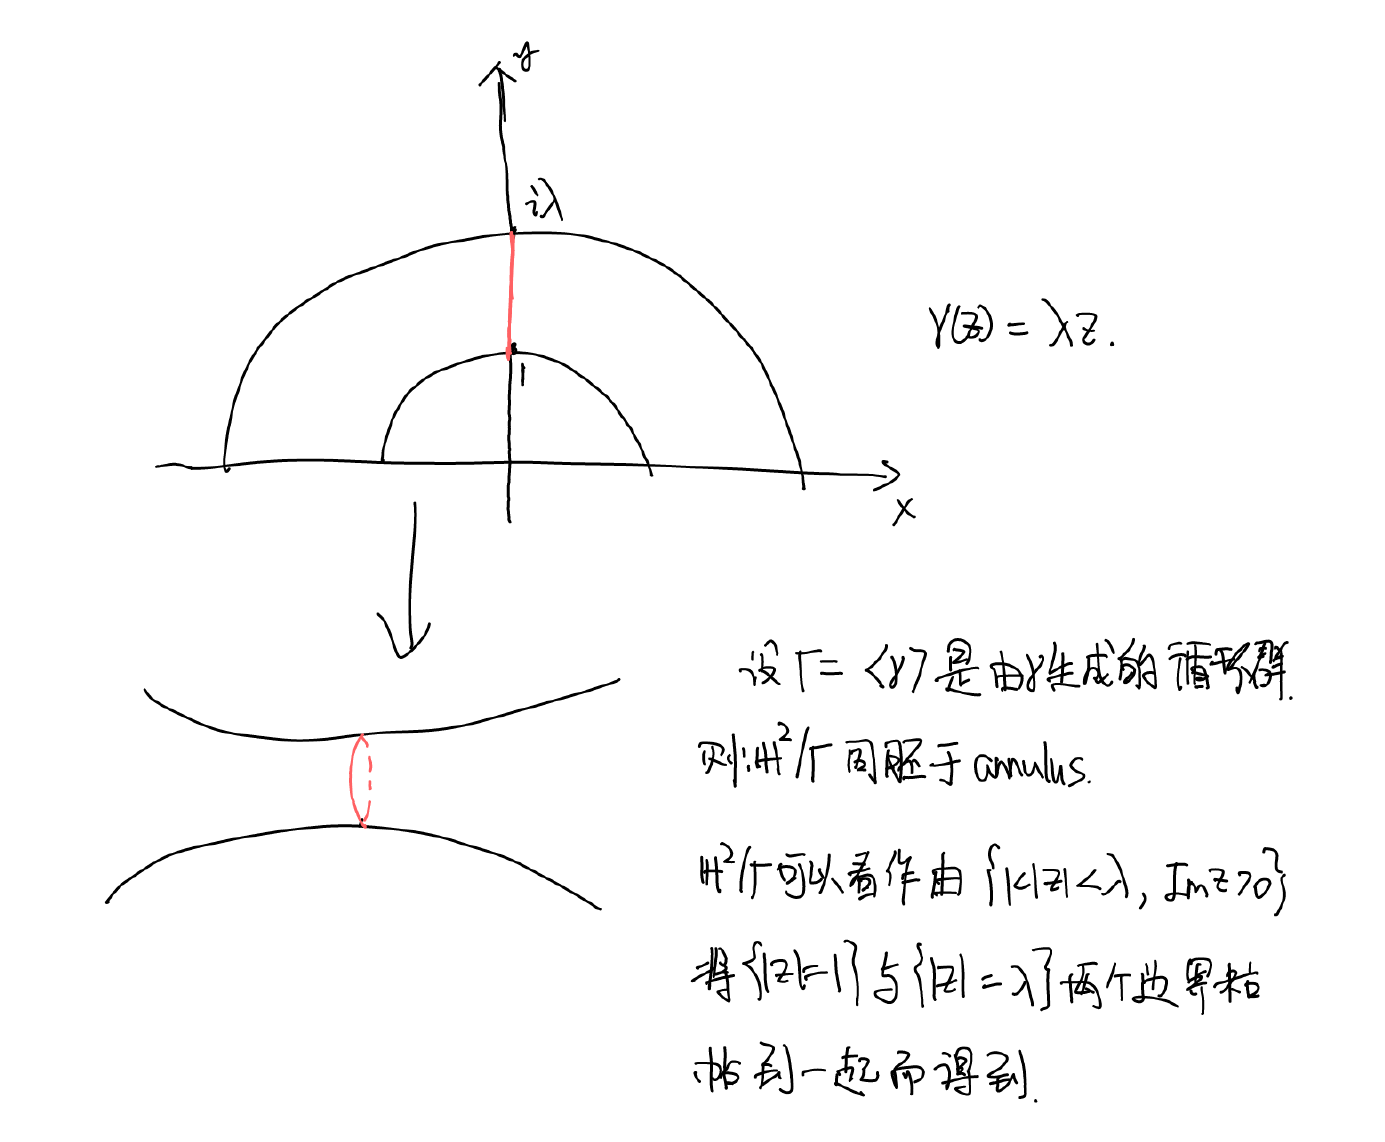
\includegraphics[scale=0.4]{images/hyperbolic_annulus.png}
    \caption{Hyperbolic Annulus}
    \label{hyperbolic_annulus}
\end{figure}

是$1-1$映射.  而$\lambda \cdot \{\abs{z}=1, \Im(z)>0\}= \{\abs{z}=\lambda, \Im(z)>0\}$. 因此, $\HH/\Gamma$可以由$\Omega_\lambda$将上下两边条边界粘贴在一起而得到. 见图\eqref{hyperbolic_annulus}. 而$\gamma$的轴投影到$\HH/\Gamma$上之后, 便成为一条闭测地线, 我们将这条闭测地线记为$\tilde{\gamma}$. 显然地, $\tilde{\gamma}$是$\pi_1(\HH/\Gamma)$的生成元. 而根据覆盖映射的性质, $\pi_1(\HH/\Gamma) = \Gamma= \left< \gamma \right>$.  因此, \textbf{$\gamma$可以自然地对应到$\tilde{\gamma}$, 后面我们将不再区分$\gamma$与$\tilde{\gamma}$}. 测地线$\tilde{\gamma}$的长度即为线段$\{\Re(z)=0, 1<\Im(z)< \lambda\}$的长度,

\begin{equation}
    l_{\tilde{\gamma}}= \int^\lambda_1 \frac{1}{y}dy=\log \lambda.
\end{equation}
我们也称$\log\lambda$为双曲型元素$\gamma$的长度.  $z \mapsto \lambda z$的矩阵表示为$\begin{pmatrix}
    &\sqrt{\lambda} \s 0 \\
    & 0 \s \rec{\sqrt{\lambda}}
\end{pmatrix}$. 于是有等式
\begin{equation}
    \begin{split}
        \text{Tr}(\begin{pmatrix}
                    &\sqrt{\lambda} \s 0 \\
                    & 0 \s \rec{\sqrt{\lambda}}
        \end{pmatrix}) = \sqrt{\lambda}+\rec{\sqrt{\lambda}} & = e^{\rec{\log \lambda}} + e^{-\rec{2}\log \lambda} \\ 
        & = 2\cosh(\frac{l_\gamma}{2}).
    \end{split}
\end{equation}
对于任意双曲型元素$\alpha \in \psl(2,\R)$, 由于$\gamma$可以共轭到$z \mapsto \lambda z$, 而在共轭作用下, 矩阵的迹是不变的.  则我们可以定义
\begin{equation}
    l_\alpha= 2\cosh^{-1}(\rec{2}\text{tr}(\alpha)).
\end{equation}
而$l_\alpha$即是$\alpha$的轴投影到曲面$\HH/\cycgroup{\alpha}$上后得到的闭测地线的长度.
\subsubsection{闭曲面上的双曲度量}
设$S_p$是亏格为$g\ge 2$的闭黎曼流形, 由等温坐标的存在性可知, $S_p$上可以赋予与黎曼度量相容的黎曼面结构. 而由单值化定理, $S_p$的万有覆盖空间同构于$\HH$(作为一个黎曼面). 由覆盖映射$\pi: \HH \to S_p$我们可以得到群嵌入$i: \pi_1(S_p) \hookrightarrow \psl(2,\R)$.  这样将$\pi_1(S_p)$看作$\psl(2,\R)$的子群后, 我们便得到了$S_p$上的双曲度量.
\begin{theorem}
    设$S_p$是亏格为$p \ge 2$的闭黎曼面. 则在其共形度量中, 存在唯一的双曲度量.
\end{theorem}
\begin{theorem}
    设$S_p$是亏格为$p \ge 2$的闭双曲曲面. 设$\alpha \subset \S_p$是一条非零伦的闭曲线. 则在$\alpha$的同伦中, 存在唯一的闭测地线.
\end{theorem}
\begin{proof}
    首先证明存在性. 设$l=\inf \{l_{\alpha'} \alpha'\text{同伦于}\alpha\}$.  取$\alpha_n$使得$\alpha_n$同伦于$\alpha$并且$l_{\alpha_n} \to l$.  取$\alpha_n$的弧长参数化, 则$\{\alpha_n\}$是等度连续逐点有界的. 则Alzera-Ascoli引理可知, 存在子列$\alpha_n \to \alpha_0$. 则$\alpha_0$是局部长度最短的, 因此是测地线.
    \par 唯一性.  设$\alpha, \beta$同两条同伦的测闭地线. 设$F(s,t): [0,1]\times \S^1 \to S_p$是$\alpha$到$\beta$的同伦.  而$[0,1]\times \S^1$的覆盖空间是$[0,1]\times \R$, 则存在覆盖提升$\tilde{F}[0,1]\times \R  \to \HH$. 即, 存在映射$\tilde{F}$使得下图可交换. 图中的$\pi$指覆盖映射的投影.
    \begin{equation}
        \begin{tikzcd}
            & {[0,1]}\times \R  \arrow{r}{\tilde{F}} \arrow{d}{\pi} &\HH \arrow{d}{\pi} \\
            & {[0,1]}\times \S^1 \arrow{r}{F}  & S_p
            \end{tikzcd}
    \end{equation}
    设$L=\sup_t l_{F(\cdot,t)}$. 则$L<+\infty$. 由于$\tilde{F}$是$F$的提升, 则$\forall t \in \R$, $l_{\tilde{F}(\cdot,t)}=l_{F(\cdot,\pi(t))}$.  $\pi(t)$表示$\R \to \S^1$的投影. 则$\forall t \in \R$, $l_{\tilde{F}(\cdot,t)}\le L$. 这意味着$d(\tilde{\alpha}, \tilde{\beta}) \le L$, 其中, $\tilde{\alpha}, \tilde{\beta}$为$\alpha,\beta$在$\HH$中的提升. 而由于双曲度量的(相对于欧氏度量)度量密度在靠近边界$\S^1$时趋近于$+\infty$, 则$d_{\R^2}(\alpha(t),\beta(t)) \overset{t\to \infty}{\longrightarrow} 0$. 于是$\tilde{\alpha}, \tilde{\beta}$是具有相同端点的测地线.  而由测地线的唯一性(推论\eqref{unique_geodesic})可知, $\tilde{\alpha}=\tilde{\beta}$. 则$\alpha=\beta$.
    \begin{figure}[!h]
        \centering
        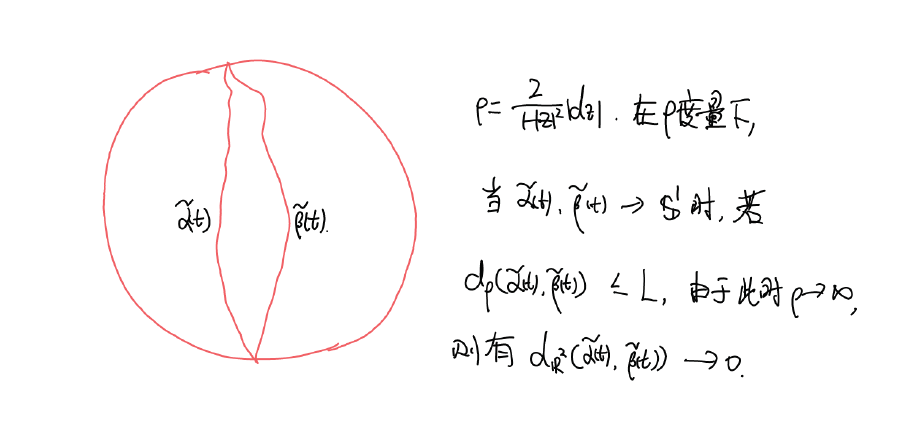
\includegraphics[scale=0.8]{images/hyper_euclidean.png}
        \caption{双曲度量与欧氏度量在$\S^1$附近的比较}
        \label{hyper_euclidean}
    \end{figure}
\end{proof}
\begin{lemma}[Collar引理] \label{collar_lemma}
    设$S_p$是亏格为$p$的双曲曲面. $\alpha, \beta \subset S_p$是简单闭测地线, 其长度分别记为$l_\alpha, l_\beta$. 设
    \begin{align}
        &\eta(l)=\rec{2}\log\frac{\cosh(\frac{l}{2})+1}{\cosh(\frac{l}{2})-1}.\\
        &\lambda(l)=\frac{4\arctan(e^{\eta(l)})-\pi}{l}.
    \end{align}
    设$A_\alpha=\{x\in S_p \mid d(x,\alpha) < l_\alpha\}$, $A_\beta=\{x \in S_p \mid d(x,\beta) <l_\beta\}$. 则
    \begin{enumerate}
        \item $A_\alpha$, $A_\beta$是嵌入annulus并且不相交. 
        \item $A_\alpha$共形同构于$\S^1 \times (0, \lambda(l_\alpha))$.
    \end{enumerate}
\end{lemma}
\begin{proof}
    设
\end{proof}
\begin{remark}
    Collar引理一般在$l$非常小的时候起作用. $l \to 0$时, $\eta(l) \sim \log \rec{l}$, $\lambda(l) \sim \frac{\pi}{l}$.
 %   我们有如下的渐近式:
 %   \begin{equation}
 %       \log\frac{x+1}{x-1} \overset{x\to 1^+}{\sim} \frac{2}{x-1}.
 %   \end{equation}
 %   \begin{equation}
 %       \frac{\cosh(x)+1}{\cosh(x)-1} \overset{x \to 0^+}{\resizebox{20em}{!}{\sim}} \frac{4}{x^2}.
 %   \end{equation}
\end{remark}
\begin{definition}
    设$S_p$是亏格为$p$的光滑曲面.  设$G$是$S_p$上所有双曲度量的集合, 赋予$C^\infty$拓扑.  在$G$上定义等价关系$\sim$: 称$g_1, g_2 \in G$等价, 当且仅当存在等距同构$f: (S_p, g_1) \to (S_p, g_2)$, 即$df^*g_2=g_1$.  定义$\M_p=G/\sim$. 称$\M_p$为曲面$S_p$的模空间.
\end{definition}
\begin{theorem}
    $\M_p$是$6p-6$维的流形.
\end{theorem}
\begin{theorem}[Mumford$\ms\ms\ms \epsilon-$紧性定理]
    设$S_p$是亏格为$p$的光滑曲面. 设$\epsilon>0$. 设
    \begin{equation}
        \M_p^\epsilon=\{g \in \M_g\mid \text{对于任意简单闭曲线}\alpha \subset S_g, l_{\alpha,g} \ge \epsilon\}.
    \end{equation}
    则$\M_p$是紧的. 其中, $l_{\alpha,g}$表示曲线$\alpha$在度量$g$下的长度.
\end{theorem}
\subsubsection{带边曲面及Schottky Double}
\begin{definition}
    设$S$是带边流形, 称$S$是带边的黎曼面, 如果存在$S$上的一组坐标卡$\{V_\alpha, \phi_\alpha\}$, 使得:
    \begin{enumerate}
        \item $\phi_\alpha$微分同胚是$\phi_\alpha: V\alpha \to \D$ 或者 $z: V \to \D \cap \{y\ge 0\}$
        \item 如果$V_\alpha \cap V_\beta \ne \emptyset$, 则$\phi_\beta \circ \phi_\alpha^{-1}$是共形映射.
    \end{enumerate}
\end{definition}
\begin{definition}
    设$S$是带边黎曼面, $\{V_\alpha, \phi_\alpha\}$是$S$上的坐标卡. 现在在$S$上定义一组新的坐标卡$\{V_\alpha, \overline{\phi}_\alpha\}$. 则在这组新的坐标卡下, $S$成为一个新的黎曼面, 记为$\overline{S}$, 并称其为$S$的镜像对称.  将$S$与$\overline{S}$的边界粘贴在一起, 就得以了一个新的黎曼面, 记为$S^d$, 称为$S$的Schottky double. 见图\eqref{fig_schottky_double}.
\end{definition}
\begin{figure}[!h]
    \centering
    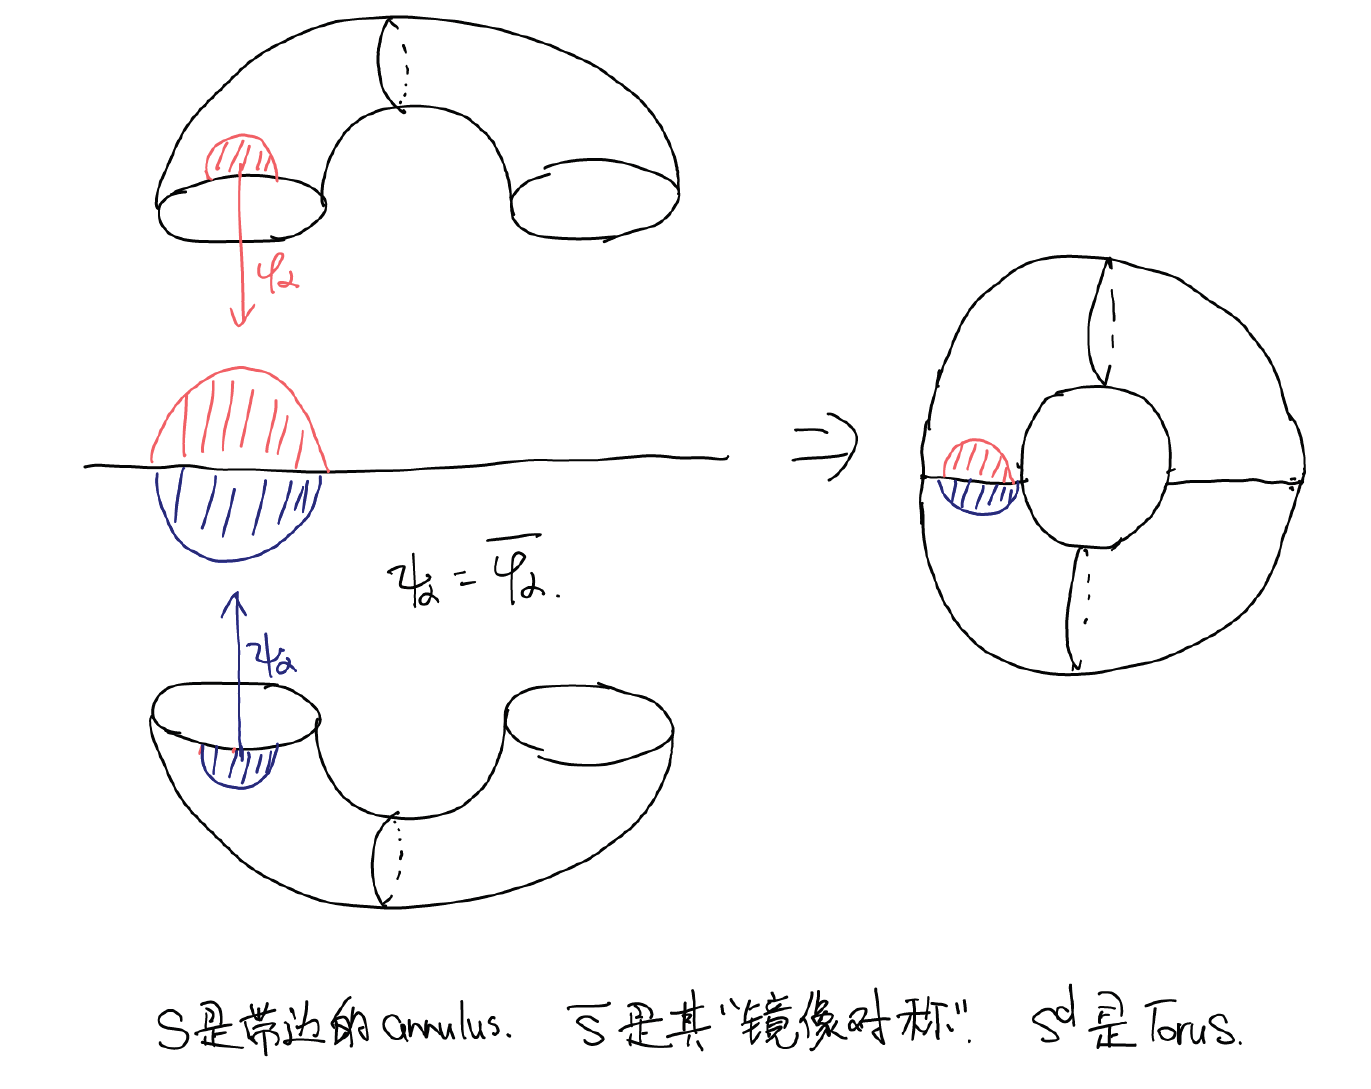
\includegraphics[scale=0.5]{images/schottky_double.png}
    \caption{Schottky double}
    \label{fig_schottky_double}
\end{figure}
借助于Schottky double, 我们可以将有关闭黎曼面的结论都推广到带边曲面上.
\begin{theorem}
    设$S_{p,k}$是亏格为$p$, 有$k$个边界的黎曼面, 并且满足$2p+k-1 \ge 2$(这只排除了非常少的情况). 则$S_{p,k}$的共形度量中, 存在唯一的双曲度量$g$, 使得$\P S_{p,k}$的每一个边界分支都是$g$度量下的闭测地线.
\end{theorem}
\begin{definition}
    设$S_{p,k}$是亏格为$p$, 有$k$个边界的光滑流形. 设$\gamma: [0,1] \to S_{p,k}$是简单光滑曲线, 且$\gamma(0), \gamma(1) \in \P S_{p,k}$, 则称$\gamma$是$S_{p,k}$中的一条简单弧.
\end{definition}
\begin{definition}
    设$\alpha, \beta \subset S_{p,k}$是简单弧. 设$\alpha$的两个端点所在的$\P S_{p,k}$的两个连通分支分别记为$\gamma_1,\gamma_2$. 称$\alpha,\beta$同伦, 如果存在映射$F(s,t):[0,1]\times [0,1] \to S_{p,k}$使得$F(0,\cdot)=\gamma, F(1,\cdot)=\beta$并且$\forall t \in [0,1], F(0,t)\in \gamma_1, F(1,t)\in \gamma_2$.
\end{definition}
\begin{lemma}
    设$S_{p,k}$是带有测地边界的双曲曲面. 设$\alpha\subset S_{p,k}$是一条简单弧. 则在$\alpha$的同伦类中, 存在唯一的测地线$\beta$, 使得$\beta$在端点处垂直于$\P S_{p,k}$.
\end{lemma}
\begin{proposition}
    设$\alpha$是$S_{p,k}$中的简单弧. 设$R_\alpha=\{x \in S_{p,k}\mid d(x,\alpha) < \eta(2l_\alpha)\}$. 则存在共形同构$\phi: R_\alpha \to [0,l_\alpha]\times (-\lambda(2l_\alpha), \lambda(2l_\alpha))$.
\end{proposition}
\begin{corollary}[带边曲面的Mumford$\ms\ms\epsilon-$紧性定理] \label{bordered_compactness}
    设$S_{p,k}$是亏格为$p$, 有$k$个边界的光滑流形. 设
    \begin{equation}
        \M_{p,k}=\{g \mid g\text{是双曲度量, 且$\P S_{p,k}$的每一个边界分支都是测地线}\}.
    \end{equation}
    设$\epsilon>0$, 设
    \begin{equation}
        \M_{p,k}^\epsilon=\{g \in \M_{p,k}\mid \text{对于任意简单闭曲线或简单弧}\alpha,\ms\ms l_{g,\alpha} \ge \epsilon\}.
    \end{equation}
    则$\M_{p,k}^\epsilon$是紧的.
\end{corollary}
\subsection{Plateau问题:The General Case}
设$S_{p,k}$是亏格为$p$, 有$k$个边界的黎曼面. 对$S_{p,k}$, 我们可以执行以下操作:
\begin{emphasize}
    设$\alpha \subset S_{p,k}$是非零伦的简单闭曲线.  将曲面$S_{p,k}$沿着$\alpha$剪开, 并在得到的两个边界上分别粘贴上两个圆盘, 得到新的曲面$S$. 如果$S$是连通的, 此时$S$的拓扑型为$(p-1,k)$. 如果曲面$S$不是连通的, 则$S$包含两个分支, 分别记为$S_{p_1,k_1}, S_{p_2,k_2}$, 满足$p_1+p_2=p, k_1+k_2=k$.
\end{emphasize}
这样的一个操作我们称为primary reduction.  曲面的集合$X=\mathop{\cup} \limits_{i=1}^{N}S_{p_i,k_i}$可以从$S_{p,k}$经过有限次primary reduction而得到, 当且仅当
\begin{equation}
    \sum p_i \le p, \sum k_i =k. 
\end{equation}
这时, 我们记为$X \prec S_{p,k}$. 
设$\Gamma=\mathop{\cup}\limits_{i=1}^{N} \gamma_i \subset \R^3$是若干条互不相交的简单闭曲线的并. 定义
\begin{equation}
    \begin{split}
        \fgg=\{u\mid & u: S_{p,k} \to \R^3, u(\P S_{p,k})= \Gamma, \text{且在$S_{p,k}$的每一个边} \\
        & \text{界分支上, $u$是单调映射}\}
    \end{split}
\end{equation}
定义
\begin{align}
    &\AA_\Gamma=\inf \{\Area(u, \rho)\mid u \in \fgg, \rho\text{是$S_{p,k}$上的双曲度量}\}.\\
    &\EE_\Gamma=\inf \{E(u, \rho)\mid u \in \fgg, \rho\text{是$S_{p,k}$上的双曲度量}\}.
\end{align}
%\chapter{黎曼流形中的Plateau问题}
%\section{调和映射}
定义
\begin{equation}
    \begin{split}
        \fgg=\{u\mid & u: X \to \R^3, u(\P X)= \Gamma, \text{且在$X$的每一个边} \\
        & \text{界分支上, $u$是单调映射}\}
    \end{split}
\end{equation}
定义
\begin{align}
    &\AA_\Gamma^*=\inf \{\Area(u, \rho)\mid u \in \fgg, \rho\text{是$X$上的双曲度量}\}.\\
    &\EE_\Gamma^*=\inf \{E(u, \rho)\mid u \in \fgg, \rho\text{是$X$上的双曲度量}\}.
\end{align}
\begin{lemma} \label{curve_small_energy}
    设$\Sigma$是带测地边界的双曲曲面. 设$u: \Sigma \to \R^3$满足 $E(u) \le K$. 设$\alpha \subset \Sigma$是非零伦的简单闭测地线. 则在$\alpha$的同伦类中, 存在简单闭曲线$\beta$, 使得
    \begin{equation}
        \int_\beta \abs{\nabla u}^2ds \le \frac{K}{\lambda(l_\alpha)}.
    \end{equation}
\end{lemma}
\begin{proof}
    由Collar引理\eqref{collar_lemma}, 存在$\alpha$的collar邻域$A_\alpha$使得$A_\alpha$是嵌入的, 且存在共形同构$\phi: \S^1 \times (0,\lambda(l_\alpha)) \to A_\alpha$. 因此,
    \begin{equation}
        E(u,A_\alpha)=E(u\circ \phi, \S^1\times (0,\lambda(l_\alpha))) \le K.
    \end{equation}
    即有
    \begin{equation}
        \int^{\lambda(l_\alpha)}_0\int_{\S^1} \abs{\nabla u\circ \phi(r,\theta)}d\theta dr \le K.
    \end{equation}
    则存在$\rho \in (0,r)$使得
    \begin{equation}
        \lambda(l_\alpha)\int_{\S^1} \abs{\nabla u\circ \phi (\rho,\theta)}^2 d\theta \le K.
    \end{equation}
    因此, 
    \begin{equation}
        \int_{\phi^{-1}(\S^1\times \{\rho\})} \abs{\nabla u}^2 d\theta \le \frac{K}{\lambda(l_\alpha)}.
    \end{equation}
    取$\beta= \phi^{-1}(\S^1 \times \{\rho\})$即可.
\end{proof}

\begin{theorem}
    如果$\AA_\Gamma < \AA_\Gamma^*$, 则存在以$\Gamma$为边界的, 同胚于$S_{p,k}$的极小曲面.
\end{theorem}
\begin{proof}
    设$u_i: \Sigma \to \R^3$, $E(u_i) \to \EE_{\Gamma}$.  记$K=\EE_{\Gamma}+1 < +\infty$. 这里, $\Sigma_i$同胚于$S_{p,k}$, 且赋予带测地边界的双曲度量$\rho_k$. 不失一般性, 可设$E(u_k) \le K$. 现在,我们证明: $\{\rho_k\}$中存在收敛子列.  由推论\eqref{bordered_compactness}, 我们只需要说明$\Sigma_k$中的简单闭曲线及简单弧的长度有严格正的下界即可.
    \begin{claim}
        存在$a>0$使得对于任意简单闭曲线$\alpha \subset \Sigma_i$, $l_\alpha \ge a$.
        \begin{subproof}
            反证法. 设存在简单闭曲线$\alpha_i\subset \Sigma_i$使得$l_{\alpha_i} \to 0$. 由引理\eqref{curve_small_energy}, 存在$\beta$同伦于$\alpha$, 且
            \begin{equation}
                \int_\beta \abs{\nabla u}^2 ds \le \frac{K}{\lambda(l_\alpha)} \to 0.
            \end{equation}
            对比不等式\eqref{annulus_small_energy}, 现在我们可以像定理\eqref{theorem_douglas_annulus}的证明中那样,构造映射$\tilde{u}_k: (\Sigma_k-\beta \cap 2\D \to \R^3$.参考图\eqref{closed_degenerate}.
        \end{subproof}
    \end{claim}
    \begin{claim}
        存在$a>0$使得对于任意简单弧$\alpha \subset \Sigma_i$, $l_\alpha \ge a$.
        \begin{subproof}
            只需要考虑$\alpha$是垂直于边界的测地线的情况即可. 这里我们分两种情况来讨论.  
            \begin{enumerate}
                \item 首先考虑$\alpha$的两个端点在$\P \Sigma_i$的不同的连通分支上. 设$d=\mathop{\min}\limits_{i\ne j} d(\gamma_i,\gamma_j)>0$. 由于$u_k(\alpha)$是连接$\Gamma$中两条曲线的弧, 则有$l_{u(\alpha)} \ge d$.  由引理\eqref{collar_arc}可知, 存在$\alpha$的邻域$V$使得存在共形同构$ \phi(s,t): (0,l_\alpha)\times (-\lambda(\frac{l_\alpha}{2}), \lambda(\frac{l_\alpha}{2})) \to V$, 并且$\phi((0,l_\alpha) \times \{0\})=\alpha$.  则由Cauchy不等式
                \begin{equation}
                    d^2 \le (\int^{l_\alpha}_0 \abs{d(u_k\circ\phi) \alpha'} ds)^2 \le l_\alpha \int^{l_\alpha}_0 \abs{d(u_k\circ \phi)}^2dr.
                \end{equation}
                于是, 有
                \begin{equation}
                    \int^{\lambda(\frac{l_\alpha}{2})}_{-\lambda(\frac{l_\alpha}{2})} \frac{d^2}{l_\alpha} \le \int^{\lambda(\frac{l_\alpha}{2})}_{-\lambda(\frac{l_\alpha}{2})} \int^{l_\alpha}_0 \abs{d(u_k\circ \phi)}^2 dtds \le E(u) \le K.
                \end{equation}
                因此, $\frac{l_\alpha}{\lambda(\frac{l_\alpha}{2})} \ge \frac{2d^2}{K}$.  由于$l\to 0$时, $\lambda(l) \to +\infty$. 则存在$a=a(d,K)>0$使得$l_\alpha \ge a$.
                \item 下面我们考虑$\alpha$的两个端点在$\P \Sigma_i$的同一个连通分支上的情况.
            \end{enumerate}
        \end{subproof}
    \end{claim}
\end{proof}